\part{FedCloud}

%%%%%%%%%%%%%%%%%%%%%%%%%%%%%%%%%%%%%%%%%%%%%%%%%%%%%%%%%%%%%%%%%%%%%%%%%%%
\begin{frame}
  \frametitle{EGI FedCloud}
  \framesubtitle{What is the EGI Federated Cloud}
    The EGI Federated Cloud is a federation of institutional private Clouds,
    offering Cloud Infrastructure as a Service to scientists in Europe
    and worldwide.

  \hfill\\

  \begin{columns}
    \column{0.7\textwidth}
        EGI Federated Cloud is based on:
        \begin{itemize}
            \item Standards and validation: federation is based on common
            Open-Standards – OCCI, CDMI, OVF, GLUE, etc...
            \item Heterogeneous implementation: no mandate on the cloud
            technology, the only condition is to expose the chosen
            interfaces and services.
        \end{itemize}

    \column{0.3\textwidth}
        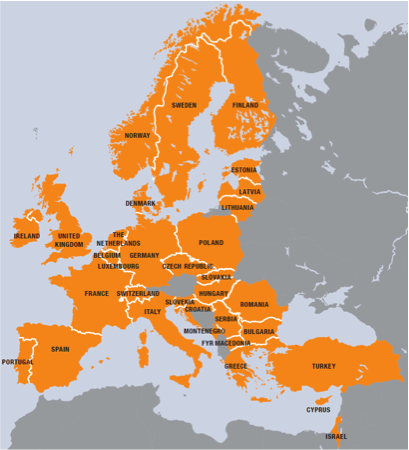
\includegraphics[width=\textwidth]{images/fedcloud_map}
  \end{columns}

  \hfill\\
      
\includegraphics[width=\textwidth]{images/fedcloud_usecases}
\end{frame}


%%%%%%%%%%%%%%%%%%%%%%%%%%%%%%%%%%%%%%%%%%%%%%%%%%%%%%%%%%%%%%%%%%%%%%%%%%%
\begin{frame}
  \frametitle{EGI FedCloud}
  \framesubtitle{Cloud Infrastructure Platform}

  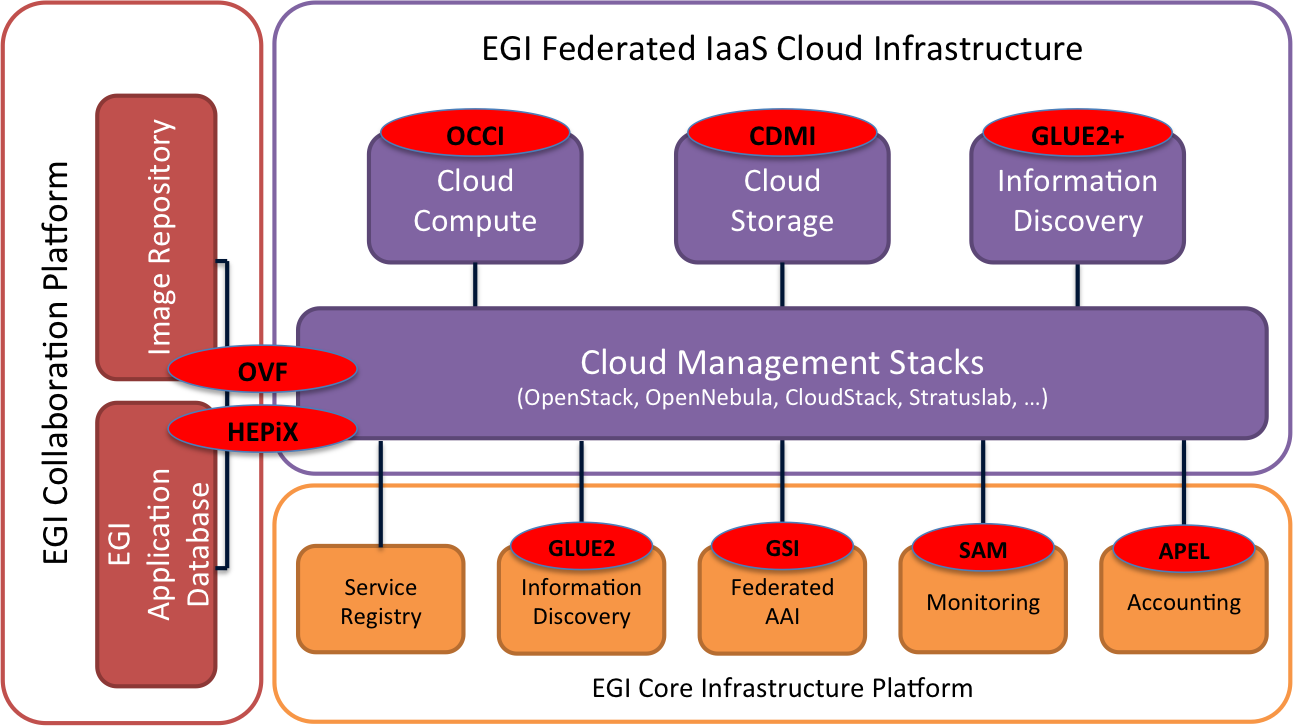
\includegraphics[width=\textwidth]{images/fedcloud_diagram}
\end{frame}

%%%%%%%%%%%%%%%%%%%%%%%%%%%%%%%%%%%%%%%%%%%%%%%%%%%%%%%%%%%%%%%%%%%%%%%%%%%
\begin{frame}
  \frametitle{EGI FedCloud}
  \framesubtitle{User workflows}

  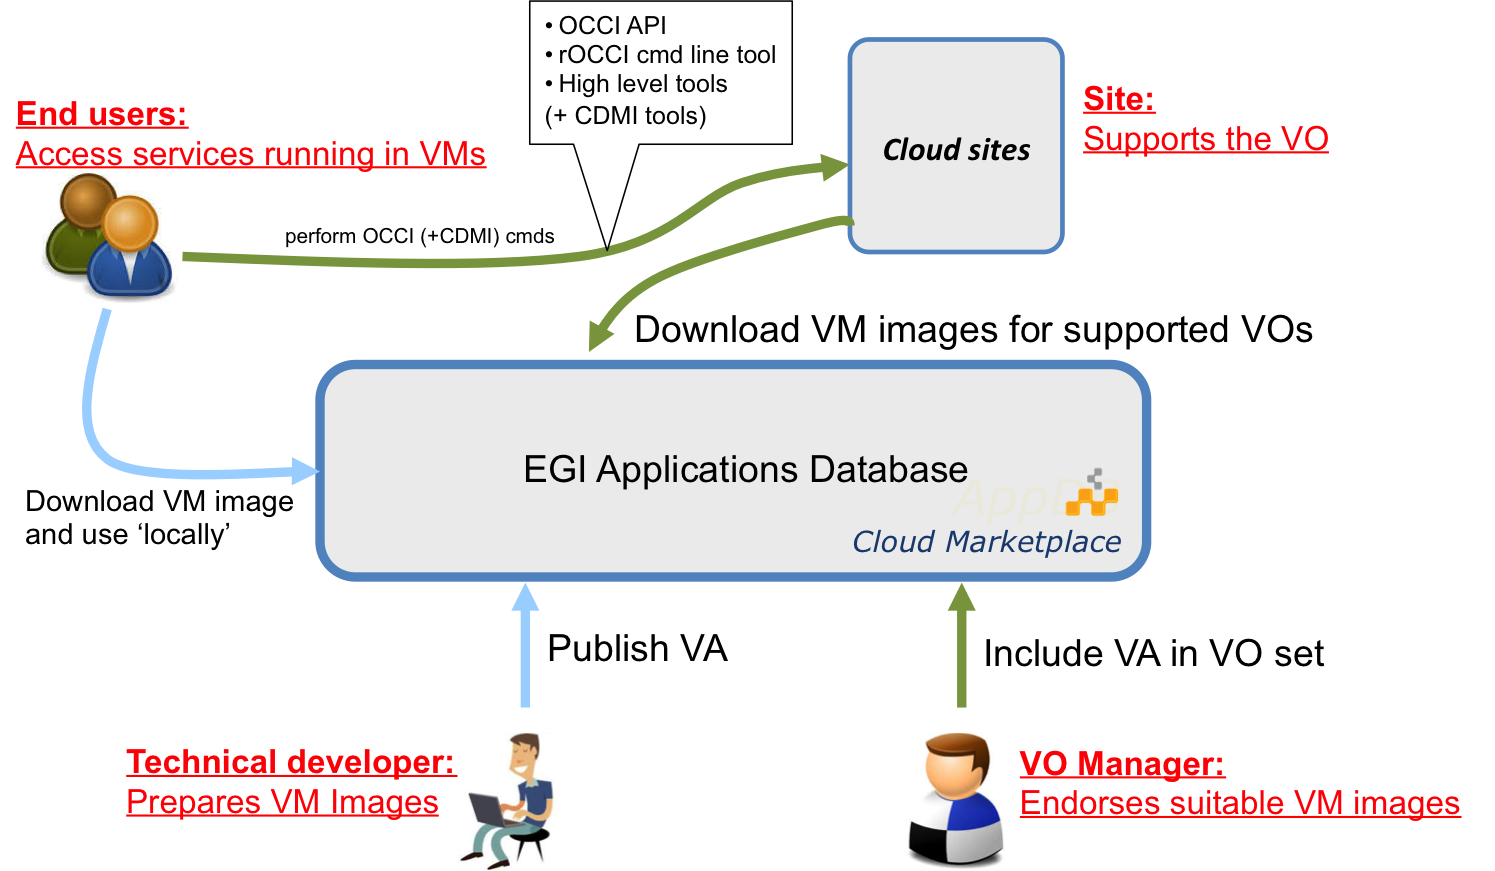
\includegraphics[width=\textwidth]{images/fedcloud_workflow}
\end{frame}

%%%%%%%%%%%%%%%%%%%%%%%%%%%%%%%%%%%%%%%%%%%%%%%%%%%%%%%%%%%%%%%%%%%%%%%%%%%

